%% =====================================================================
%%  International Journal of Control, Automation, and Systems (IJCAS)
%%  Manuscript: Learned Direct Actuation versus Tuned and RL-Tuned
%%              Pure Pursuit: A Controlled Comparison for Path Tracking
%%  Self-contained source reproducing the IJCAS two-column layout.
%%  Compile with:  pdflatex manuscript.tex   (run twice)
%%  Figure files expected in the same folder (or ./figures, see below):
%%    fig01_overview.png  fig02_inputs.png     fig03_circuits.png
%%    fig04_accuracy.png  fig05_laps.png       fig06_cdf.png
%%    fig07_montreal_zoom.png fig08_lookahead.png fig09_training.png
%%    fig10_laptime.png   fig11_rlpp_schedule.png
%% =====================================================================
\RequirePackage{fix-cm}
\documentclass[10pt,twocolumn,twoside]{article}

%% ---------- Page geometry (IJCAS trim: 210 x 280 mm) ----------------
\usepackage[paperwidth=210mm,paperheight=280mm,
            left=20mm,right=20mm,top=17mm,bottom=26mm,
            headheight=22pt,headsep=5mm,footskip=12mm,
            columnsep=6mm]{geometry}

%% ---------- Fonts and symbols ----------------------------------------
\usepackage[T1]{fontenc}
\usepackage{times}               % Times text, Computer Modern math
\usepackage{amsmath,amssymb,bm}
\usepackage{textcomp}

%% ---------- Graphics, colours, tables ----------------------------------
\usepackage{graphicx}
\graphicspath{{./}{./figures/}}
\usepackage[table]{xcolor}
\usepackage{booktabs,multirow,array,tabularx}
\usepackage{stfloats}            % allows figure*[b] / table*[b]
\usepackage{algorithm}
\usepackage[noend]{algpseudocode}
\usepackage{enumitem}
\usepackage{cite}
\usepackage[hyphens]{url}
\urlstyle{same}

%% ---------- IJCAS colours ----------------------------------------------
\definecolor{ijblue}{rgb}{0.275,0.494,0.651}
\definecolor{ijorange}{rgb}{0.890,0.424,0.039}

%% ---------- Captions ("Fig. 1." / "Table 1." in blue) -----------------
\usepackage{caption}
\DeclareCaptionLabelFormat{ijcas}{#1~#2.}
\captionsetup{font=normalsize,labelfont={color=ijblue},labelformat=ijcas,
              labelsep=space,format=hang,justification=justified,
              singlelinecheck=false,skip=4pt}
\captionsetup[figure]{name=Fig.,margin={0pt,6pt}}
\captionsetup[table]{name=Table,position=top}

%% ---------- Section headings -------------------------------------------
\usepackage{titlesec}
\titleformat{\section}[block]
  {\centering\normalsize\bfseries\color{ijblue}}
  {\thesection.}{0.6em}{\MakeUppercase}
\titlespacing*{\section}{0pt}{12pt plus 2pt}{8pt plus 1pt}
\titleformat{\subsection}[block]
  {\fontsize{10.5}{12.5}\selectfont\color{ijblue}}
  {\thesubsection.}{0.5em}{}
\titlespacing*{\subsection}{0pt}{9pt plus 2pt}{5pt plus 1pt}
\newcommand{\parhead}[1]{\textbf{#1}\hspace{0.4em}}

%% ---------- Running heads ----------------------------------------------
\newcommand{\shorttitle}{Learned Direct Actuation versus Tuned and RL-Tuned Pure Pursuit}
\newcommand{\shortauthors}{Piyush Joshi, Dileep Banothu, N. Sanjay Varma and Atin Chowdhury}
\usepackage{fancyhdr}
\pagestyle{fancy}
\fancyhf{}
\renewcommand{\headrulewidth}{0pt}
\fancyhead[LE]{\small\thepage}
\fancyhead[CE]{\small\shortauthors}
\fancyhead[CO]{\small\shorttitle}
\fancyhead[RO]{\small\thepage}
\fancypagestyle{ijcasfirst}{%
  \fancyhf{}%
  \fancyhead[L]{\footnotesize Manuscript submitted for peer review}%
  \fancyhead[R]{\footnotesize \thepage}%
  \renewcommand{\headrulewidth}{0pt}}

%% ---------- Lists, spacing ----------------------------------------------
\setlist[itemize]{leftmargin=1.2em,itemsep=1pt,topsep=3pt,parsep=0pt,label=\textbullet}
\setlength{\parindent}{1.2em}
\setlength{\textfloatsep}{10pt plus 2pt minus 2pt}
\setlength{\dbltextfloatsep}{10pt plus 2pt minus 2pt}
\setlength{\abovedisplayskip}{6pt plus 2pt minus 2pt}
\setlength{\belowdisplayskip}{6pt plus 2pt minus 2pt}
\renewcommand{\topfraction}{0.9}
\renewcommand{\dbltopfraction}{0.9}
\renewcommand{\textfraction}{0.07}
\renewcommand{\floatpagefraction}{0.85}
\renewcommand{\dblfloatpagefraction}{0.85}

%% ---------- Hyperlinks (blue citations as in IJCAS) ---------------------
\usepackage[colorlinks=true,linkcolor=ijblue,citecolor=blue,urlcolor=black]{hyperref}

%% ---------- Notation -----------------------------------------------------
\newcommand{\vmatch}{v_{\mathrm{match}}}
\newcommand{\amax}{a_{\max}}
\newcommand{\vmax}{v_{\max}}
\newcommand{\Ld}{L_d}
\newcommand{\geom}[1]{\mathrm{Geom}@#1}
\newcommand{\dpo}{DAgger$\to$PPO}
\newcommand{\one}{\mathbf{1}}

%% =========================================================================
\begin{document}

\twocolumn[{%
\thispagestyle{ijcasfirst}
\begin{flushleft}
\vspace*{2pt}
{\fontsize{15.4}{18.5}\selectfont\bfseries\color{ijblue}
Learned Direct Actuation versus Tuned and RL-Tuned Pure Pursuit: A\\
Controlled Comparison for Path Tracking\par}
\vspace{6pt}
{\normalsize\bfseries Piyush Joshi, Dileep Banothu, N.\ Sanjay Varma and Atin Chowdhury\par}
\end{flushleft}
\vspace{2pt}
\noindent\rule{\textwidth}{0.4pt}\par
\vspace{8pt}
\begin{list}{}{\leftmargin=12pt\rightmargin=12pt\itemsep=0pt\topsep=0pt}
\item[]\textbf{\color{ijorange}Abstract:}
Two parameters govern Pure Pursuit (PP) tracking, its steering gain and its
lookahead distance, and reinforcement learning (RL) has recently been
integrated with PP by letting an agent tune both online. We compare such integration of learning with
classical control against learning that replaces the geometric law. A network controls a point-mass ``bead'' along image-extracted references
using imitation learning (DAgger), PPO, or both. It is compared with tuned PP, an adaptation of RL-tuned PP, and
the PP law run on the bead, under one simulator and lap rule, on eight held-out
F1TENTH circuits with five training seeds. Imitating a hand-written rule, the
bead matches that rule (1.06~cm RMSE). With our PPO budget and settings, PPO
did not improve this imitation policy. Tuned PP reaches 0.31~cm at the bead's
speed, and 0.28~cm when run on the bead, so the gap stems from the control law,
not the vehicle; against the true centerlines it shrinks from 0.75 to 0.36~cm
but keeps its sign. Imitating the PP law instead, the network reaches 0.42~cm
and matches tuned PP against the true centerlines. On a dynamic single-track
car, gains must be re-tuned; PP then stays the most accurate car controller
(1.83~cm), its lead over Stanley being clear with tyres only and unclear with a
steering-rate limit. A naive protocol with test
leakage and untuned baselines would reverse these conclusions.
\vspace{8pt}
\item[]\textbf{\color{ijorange}Keywords:} Pure pursuit, path tracking,
imitation learning, reinforcement learning, F1TENTH.
\end{list}
\vspace{6pt}
\noindent\rule{\textwidth}{0.4pt}\par
\vspace{14pt}
}]

%% Affiliation block at the foot of page 1 (full width)
\begin{figure*}[b]
\hrule height 0.5pt
\vspace{6.5pt}
{\fontsize{8.5}{10}\selectfont\leftskip=3.6pt\rightskip=3.6pt\noindent
Piyush Joshi, Dileep Banothu, N.\ Sanjay Varma and Atin Chowdhury are with
the Department of Computer Science and Engineering, Indian Institute of
Information Technology Sri City, Sri City, Andhra Pradesh 517646, India
(e-mails: piyush.j@iiits.in, dileep.b24@iiits.in, sanjayvarma.n24@iiits.in,
atin.c23@iiits.in).\par}
\vspace{4.5pt}
\hrule height 0.5pt
\end{figure*}

%% =========================================================================
\section{Introduction}

Between the planner and the actuators of an autonomous vehicle sits a path
tracker, which converts the planned path into motion commands. On small-scale
racing cars such as F1TENTH~\cite{okelly2020f1tenth} the tracker is typically
geometric, and Pure Pursuit (PP)~\cite{coulter1992,snider2009} is the most
common choice: it aims at the path point lying a lookahead distance $\Ld$ ahead
and scales the resulting steering by a gain $g$. The choice of $\Ld$ is a
compromise---a small value responds fast but oscillates, a large value is
smooth but cuts corners.

Computational intelligence can be integrated with such a controller in two
ways. In RL-tuned PP~\cite{elgouhary2026}, an agent trained
with Proximal Policy Optimization (PPO)~\cite{schulman2017ppo} selects
$(\Ld,g)$ online while the PP law
stays in the loop---learning \emph{inside} classical control. The alternative
replaces the law: a network outputs the actuation itself and can be trained by
imitation of a teacher, by reinforcement learning (RL), or both. Whether the
second route is more precise is rarely tested under identical conditions.

We run that test with a ``bead'', a point mass following references
extracted from images, and design the comparison against three confounds. Test
leakage and untuned baselines can make a learned controller look better than it
is, so the test circuits stay out of training, selection and tuning, every
baseline is tuned until its optimum lies inside the searched range, and the
imitated teacher is reported. The vehicle can matter as much as the
controller---the bead accelerates in any direction, the PP car must steer---so
both plants share one lap rule and the PP law is also run on the bead. And the
extracted reference has its own error, so all results are also measured against
the true circuit centerlines.

Our contribution is the controlled comparison and its findings:
\begin{itemize}
\item a comparison of a direct-actuation network trained by
  DAgger~\cite{ross2011dagger}, by PPO and by DAgger-initialized PPO with tuned
  PP and an adaptation of RL-tuned PP~\cite{elgouhary2026}, with one simulator,
  one lap rule and one metric code, at native and matched speed;
\item same-plant controls---the PP law on the bead, the expert aiming further
  ahead, and DAgger with the PP law as teacher---that separate the control law,
  the vehicle and the teacher;
\item the finding that, on the kinematic car and on the bead, a well-tuned PP
  law is more accurate than every learned controller that does not imitate it;
  that the imitation
  policy is limited mainly by its teacher, matching tuned PP on the real track
  only when taught by the PP law; and that, with our budget and settings, PPO
  did not improve it;
\item a tuned Stanley baseline, and a dynamic single-track check at matched
  speed where the geometric laws are re-tuned and RL--PP is retrained;
\item a naive-protocol contrast that shows how test leakage and untuned
  baselines would have reversed these conclusions.
\end{itemize}

%% ---------------- Fig. 1 -------------------------------------------------
\begin{figure}[t]
\centering
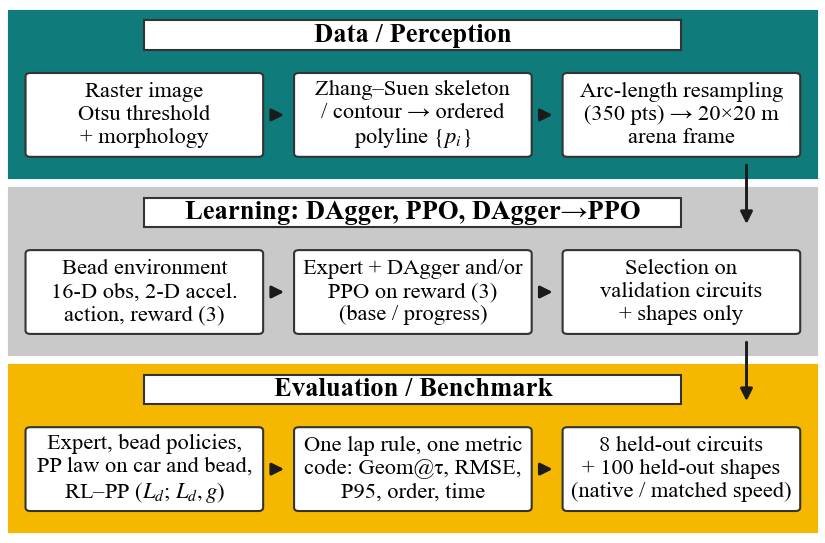
\includegraphics[width=\columnwidth]{fig01_overview}
\caption{System overview: image to ordered reference path; bead network
trained by DAgger, PPO or DAgger$\to$PPO with selection on validation paths;
all controllers scored with one lap rule and one metric code on circuits and
shapes kept out of training.}
\label{fig:overview}
\end{figure}

%% ---------------- Table 1 ------------------------------------------------
\begin{table}[t]
\caption{Waypoint spacing of the extracted circuit references (median and
range of the distance between consecutive waypoints).}
\label{tab:spacing}
\centering
\resizebox{\columnwidth}{!}{%
\begin{tabular}{@{}lcccc|lcccc@{}}
\toprule
Circuit & Split & $N$ & Median & Range & Circuit & Split & $N$ & Median & Range \\
 & & & [cm] & [cm] & & & & [cm] & [cm] \\
\midrule
BrandsHatch   & train & 350 & 20.1 & 19.6--21.6 & Shanghai    & val  & 350 & 21.7 & 20.3--23.1 \\
Budapest      & train & 350 & 17.7 & 16.7--18.5 & Spa         & val  & 350 & 16.6 & 15.0--17.8 \\
Catalunya     & train & 350 & 19.5 & 18.3--20.9 & Spielberg   & val  & 350 & 16.6 & 5.6$^{\ddagger}$--17.7 \\
IMS           & train & 350 & 13.3 & 12.3--13.3 & Austin      & test & 350 & 14.6 & 10.5$^{\ddagger}$--15.6 \\
MexicoCity    & train & 349 & 14.6 & 13.3--15.4 & Hockenheim  & test & 350 & 15.1 & 14.1--16.1 \\
MoscowRaceway & train & 350 & 16.5 & 15.9--17.5 & Montreal    & test & 350 & 11.1 & 10.7--11.8 \\
Nuerburgring  & train & 350 & 16.5 & 16.1--17.5 & Monza       & test & 350 & 13.0 & 12.2--13.6 \\
Oschersleben  & train & 350 & 17.4 & 17.0--18.4 & Silverstone & test & 350 & 16.6 & 16.1--17.6 \\
Sakhir        & train & 350 & 21.9 & 20.3--23.0 & Sochi       & test & 350 & 15.4 & 14.3--16.5 \\
SaoPaulo      & train & 350 & 19.9 & 19.7--21.3 & YasMarina   & test & 350 & 15.1 & 13.3--16.1 \\
Sepang        & train & 350 & 23.5 & 21.8--24.6 & Zandvoort   & test & 350 & 21.5 & 20.4--23.0 \\
Melbourne     & val   & 350 & 14.7 & 12.9--15.5 & & & & & \\
\bottomrule
\end{tabular}}

\vspace{3pt}
\parbox{\columnwidth}{\fontsize{8}{9.5}\selectfont
$^{\ddagger}$Shortest segment is the last one, where the extracted loop stops
short of its start and its final points hook back slightly; it is not a
junction between pieces (no circuit reference has a break): Spielberg 5.6~cm,
loop open by 8.2~cm, minimum of the other segments 15.7~cm; Austin 10.5~cm, loop
open by 4.6~cm, minimum of the other segments 12.9~cm.}
\end{table}

%% =========================================================================
\section{Related Work}

\parhead{Geometric trackers.}Among geometric path followers~\cite{snider2009},
Pure Pursuit~\cite{coulter1992} and the Stanley controller~\cite{hoffmann2007}
are the most widely used; the kinematic and dynamic models behind them are
treated in~\cite{rajamani2012,kong2015}. A family of PP variants schedules $\Ld$
with speed or curvature through hand-designed rules. In racing, the reference
line itself is often obtained by minimizing
curvature~\cite{heilmeier2020,betz2022}.

\parhead{Learned control.}Deep RL is widely applied, as surveys show
for driving~\cite{kiran2022} and for robot control~\cite{kober2013}.
PPO~\cite{schulman2017ppo}, usually paired with GAE (Generalized Advantage
Estimation)~\cite{schulman2016gae}, is a common on-policy algorithm whose
outcome is sensitive to implementation details~\cite{andrychowicz2021};
SAC~\cite{haarnoja2018} and other off-policy algorithms need fewer samples. End-to-end policies gain
flexibility at the cost of interpretability and transfer~\cite{evans2023},
whereas RL tuning of a classical controller~\cite{elgouhary2026} keeps the
controller in the loop.

\parhead{Imitation learning.}Learning to drive from demonstrations dates back
to ALVINN~\cite{pomerleau1989}. DAgger~\cite{ross2011dagger} limits the growth
of errors over time by having the teacher label whatever states the learner
visits. Since imitation tends toward the teacher's own performance, getting
beyond it usually takes RL fine-tuning.

%% =========================================================================
\section{Methods}

Fig.~\ref{fig:overview} outlines the system.

\subsection{Reference extraction}

An input image is first reduced to at most 1200~px on its longer side, turned
into gray scale and blurred with a Gaussian kernel. A global Otsu
threshold~\cite{otsu1979} then splits stroke from background, with the polarity
taken from the median gray level of the border pixels, and a $3\times3$
morphological closing removes small gaps. A drawing occupying no more than a
fifth of the image is thinned to single-pixel width with the Zhang--Suen
algorithm~\cite{zhang1984}; bigger regions are followed along their outer
boundary. The pixels of each 8-connected skeleton piece are put in order by a
walk that starts at one end and, at a branch, takes the neighbour with the
smallest change of direction. After scaling to a $20\times20$~m arena, any
piece under 0.1~m is discarded and the others share about 350 equally spaced
points; no distance computation crosses the breaks between pieces. Images without a valid path are reported as failures,
never replaced by a default path. Each circuit image is drawn from a centerline
we know, which makes the extraction error directly measurable: per circuit, the
extracted reference lies on average 0.79--1.24~cm from the source centerline,
and at most 6.53~cm. Rasterization also shrinks the F1TENTH tracks by a linear
factor of 4.3--9.8 (median 6.5), to 39--82~m, and the spacing of the extracted
waypoints is 11.1--23.5~cm per circuit (median 16.6~cm;
Table~\ref{tab:spacing}). Four sample inputs and their paths appear in
Fig.~\ref{fig:inputs}.

%% ---------------- Fig. 2 -------------------------------------------------
\begin{figure}[t]
\centering
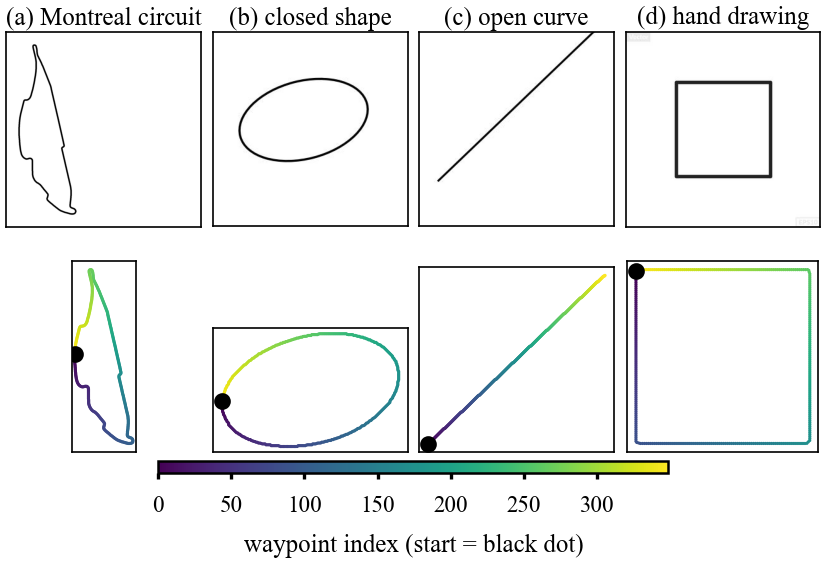
\includegraphics[width=\columnwidth]{fig02_inputs}
\caption{From image to reference path. Upper row: four inputs, namely one test
circuit rendered as an image, one closed and one open synthetic test contour,
and a hand drawing. Lower row: the ordered paths obtained from them, shaded by
waypoint number, with waypoint 0 shown as a black dot.}
\label{fig:inputs}
\end{figure}

\subsection{Bead dynamics, observation and reward}

The bead is modelled as a point mass with position $\mathbf{p}_t$, velocity $\mathbf{v}_t$
and command $\mathbf{u}_t\in[-1,1]^2$, scaled to at most $\amax=10$~m/s$^2$ per
axis, with viscous friction $\mu=7$~s$^{-1}$, $\vmax=7$~m/s and
$\Delta t=0.016$~s:
\begin{equation}
\begin{aligned}
\mathbf{v}_{t+1} &= (\mathbf{v}_t+\amax\mathbf{u}_t\Delta t)(1-\mu\Delta t),\\
\mathbf{p}_{t+1} &= \mathbf{p}_t+\mathbf{v}_{t+1}\Delta t.
\end{aligned}
\label{eq:bead}
\end{equation}
Full actuation along a single axis yields the steady speed
$v^{*}=\amax\Delta t(1-\mu\Delta t)/(\mu\Delta t)\approx1.27$~m/s. A waypoint
counter $w_t$ may move ahead by four indices or fewer in one step, and only onto
points closer than $\rho=0.18$~m; a lap is finished when $w_t$ reaches 99\% of
the path, and episodes end after
$\max(3500,\lceil1.5L/(v^{*}\Delta t)\rceil)$ steps for a path of length $L$ or
after 400 steps without progress. The PP car uses the same counter code, lap
rule, stall rule and step cap.

The policy observes 16 values scaled to $[-1,1]$ by construction (vectors to
waypoints $w_t$, $w_t+1$ and $w_t+5$, position, velocity and heading, the
distance to the path, an on-path flag, a curvature measure and the completed
fraction), so no running input normalization is used. With $e_t$ the gap
to the closest point of the reference, $d_t$ the gap to waypoint $w_t$, $n_t$ the
waypoints passed in step $t$ and $\hat{\mathbf{r}}_t$ the path tangent, the
reward is
\begin{equation}
\begin{aligned}
r_t ={}& 0.1\,\mathrm{clip}\big((d_{t-1}-d_t)/\rho,\pm1\big)+0.4\,n_t\\
 &+0.25\,e^{-(e_t/0.08)^2}+0.15\,\mathrm{clip}(\mathbf{v}_t\cdot\hat{\mathbf{r}}_t/\vmax,\pm1)\\
 &-0.05\min(e_t/0.1,3)-0.1\cdot\one[e_t>\rho]\\
 &-0.05\cdot\one_{\mathrm{back}}-0.5\cdot\one_{\mathrm{wall}}\\
 &-0.005\min(\|\mathbf{u}_t-\mathbf{u}_{t-1}\|,1)-0.001,
\end{aligned}
\label{eq:reward}
\end{equation}
plus $+50$ for a finished lap, $+15$ for a truncated episode past 80\% and $-5$
otherwise; the weights were set before the data split and not tuned. Because
every step pays the centering bonus, a slower lap earns more of it:
adding Gaussian noise of standard deviation 0.61 to the expert's actions triples
its validation RMSE (0.91 to 2.92~cm) yet raises its return from 746 to 764. A
progress variant therefore pays the bonus per waypoint passed,
$2.0\,n_te^{-(e_t/0.08)^2}$, keeping its per-lap budget at the expert's pace;
the noisy expert then earns less than the noise-free one (725 versus 836).

\subsection{Learning the bead controller}

All bead policies share one actor--critic architecture, implemented in
Stable-Baselines3~\cite{raffin2021sb3}: actor and critic are separate two-layer
$\tanh$ networks with 256 units per layer, and actions are sampled from a Gaussian
with state-independent spread. During testing the mean action is
executed. The hand-written expert steers toward the next waypoint,
\begin{equation}
\mathbf{u}^{*}_t=\big(\mathbf{p}[w_t+1]-\mathbf{p}_t\big)\big/\big\|\mathbf{p}[w_t+1]-\mathbf{p}_t\big\|.
\label{eq:expert}
\end{equation}
Bead-DAgger first regresses the actor on a single teacher episode for each
training path and refines it with DAgger (Algorithm~\ref{alg:dagger}); the reward is not used. The teacher
is the expert~\eqref{eq:expert} or, in Bead-DAgger (Bead-PP teacher), the PP law
run on the bead (Section~\ref{sec:beadpp}).

Bead-PPO trains the same network from a random initialization by maximizing the
clipped PPO objective,
\begin{equation}
L(\theta)=\mathbb{E}_t\big[\min\big(\rho_t\hat A_t,\ \mathrm{clip}(\rho_t,1\pm\varepsilon)\hat A_t\big)\big]-c_vL^{V}+c_eH,
\label{eq:ppo}
\end{equation}
with GAE advantages~\cite{schulman2016gae}, for $3\times10^{6}$ steps. The
starting value $\log\sigma_0=-0.5$ of the policy's log standard deviation was
picked among $\{-1,-0.5,0\}$ by a pilot with seed 100 scored on validation
references only (scores 0.750, 0.851 and 0.811 after $7.5\times10^{5}$ steps).

Bead-\dpo{} starts from the expert-taught DAgger actor with the same seed,
holds that actor fixed for $5\times10^{4}$ steps while only the critic learns,
and continues with~\eqref{eq:ppo} for $2\times10^{6}$ steps. To avoid scrambling the initial
policy it starts with $\log\sigma_0=-2$, uses the learning rate $10^{-4}$, and
adds a behaviour-cloning term
\begin{equation}
L_{\mathrm{BC}}(\theta)=\lambda\,\mathbb{E}_t\big[\|\mu_\theta(o_t)-\mathbf{u}^{*}_t\|^2\big],\quad\lambda=1,
\label{eq:bc}
\end{equation}
where $\mu_\theta$ is the actor mean and $\mathbf{u}^{*}_t$ is recovered exactly
from the observation. Both PPO procedures are run with the base and the
progress reward.

Each variant learns on the training split, and its final checkpoint is the one
scoring highest on validation; the score is average $\geom{0.10}$ (as a
fraction) less average RMSE (in meters), averaged over validation circuits and
shapes. In these units 1~cm of
RMSE weighs as much as one percentage point of coverage; RMSE alone does not
notice skipped sections, which $\geom{0.10}$ penalizes. Selecting by RMSE alone
would have chosen the same checkpoint or setting in 32 of 45 runs and grids, and
otherwise a validation RMSE within 0.48~cm. Hyper-parameters are listed in
Table~\ref{tab:hyper}.

%% ---------------- Table 2 ------------------------------------------------
\begin{table}[t]
\caption{Learning hyper-parameters.}
\label{tab:hyper}
\centering
\resizebox{\columnwidth}{!}{%
\begin{tabular}{@{}lll@{}}
\toprule
Quantity & Bead (PPO variants) & RL--PP (adaptation of~\cite{elgouhary2026})\\
\midrule
MLP (policy/value) & $[256,256]$ $\tanh$ & $[64,64]$ $\tanh$\\
$n_{\mathrm{steps}}$ / batch / epochs & $2048\times4$ envs / 128 / 10 & 2048 / 256 / 5\\
$\gamma$ / GAE $\lambda$ / clip & 0.99 / 0.95 / 0.2 & 0.99 / 0.98 / 0.2 (KL 0.015)\\
Entropy / value coeff. & 0.001 / 0.5 & 0.02 / 0.6\\
Learning rate & $3\times10^{-4}$; fine-tune $10^{-4}$ & $2.4\times10^{-4}$, linear decay\\
Initial $\log\sigma$ & $-0.5$; fine-tune $-2$ & 0\\
BC weight $\lambda$ & fine-tune 1 (check: 0.1, 10) & --\\
Normalization & none (inputs in $[-1,1]$) & VecNormalize (obs., return)\\
Steps per run & $3\times10^{6}$; fine-tune $2\times10^{6}$ & $10^{5}$\\
Training seeds & 0--4 & 0--4\\
\bottomrule
\end{tabular}}
\end{table}

\subsection{Pure Pursuit baselines}

The PP car is a kinematic bicycle~\cite{rajamani2012} with wheelbase
$W=0.33$~m. With $y'$ the sideways offset, in the car's frame, of the
lookahead point,
\begin{equation}
\begin{aligned}
\gamma &= g\cdot2y'/\Ld^{2}, \qquad \dot\theta=(v/W)\tan\delta,\\
\delta &= \mathrm{clip}\big(\arctan(W\gamma),\pm1.10~\mathrm{rad}\big).
\end{aligned}
\label{eq:pp}
\end{equation}
Speed follows $v_{\mathrm{ref}}=\mathrm{clip}\big(4.2/\sqrt{1+2.5|\kappa|},1.8,5.0\big)$~m/s
with braking and acceleration passes. The model has no tyre forces: at native
speed, tuned PP demands more than 10~m/s$^2$ of lateral acceleration in 12.4\%
of its test steps, which a real car could not sustain; at the matched speed
below, the maximum is 9.4~m/s$^2$.

%% ---------------- Algorithm 1 --------------------------------------------
\begin{algorithm}[t]
\caption{DAgger for the bead (Bead-DAgger).}
\label{alg:dagger}
\small
\begin{algorithmic}[1]
\State \textbf{Input:} training paths $\mathcal{T}$, validation paths
  $\mathcal{V}$, teacher $\pi^{*}$, network $\pi_\theta$,
  $\beta=(0.4,0.2,0.1,0.05,0,0,0,0)$
\State $\mathcal{D}\gets$ one teacher episode per $\tau\in\mathcal{T}$; fit actor
  on $\mathcal{D}$ (12 epochs, lr $2\times10^{-4}$)
\For{round $k=1,\dots,8$}
  \State for each $\tau\in\mathcal{T}$ roll out one episode; at every step
    execute $\pi^{*}$ with probability $\beta_k$, else $\pi_\theta$, and label
    the state with $\pi^{*}(o)$
  \State $\mathcal{D}\gets\mathcal{D}\cup\{(o,\pi^{*}(o))\}$; refit actor
    (8 epochs, lr $1.5\times10^{-4}$ for $k\le3$, else $7\times10^{-5}$)
  \State keep the checkpoint if the validation score on $\mathcal{V}$ improves
\EndFor
\State \Return best validation checkpoint
\end{algorithmic}
\end{algorithm}

Fixed and Adaptive PP use constant $(\Ld,g)$ and
$\Ld=\mathrm{clip}(a+bv,0.05,1.20)$ with $g=1.05$. Both are tuned by grid search over
the training references, using the selection score above, over
$\Ld\in\{0.05,0.075,\dots,0.20\}\cup\{0.25,0.30,\dots,1.00\}$~m,
$g\in\{0.6,\dots,1.4\}$, $a\in\{0,0.025,\dots,0.5\}$ and
$b\in\{0,0.025,0.05,\dots,0.25\}$~s. Fixed PP selects $(0.125~\mathrm{m},0.9)$
at native and $(0.125~\mathrm{m},1.0)$ at the matched speed, inside the grid
(training RMSE 0.37, 0.24 and 0.26~cm at 0.10, 0.125 and 0.15~m). Adaptive PP
selects $(a,b)=(0.05,0.025)$, but the best constant lookahead scores within
0.001~cm, so it is in effect a Fixed PP.

Stanley~\cite{hoffmann2007} runs on the same car:
$\delta=\psi_{\mathrm{path}}-\psi+\arctan\big(k\,e_f/(k_s+v)\big)$, clipped to
$\pm1.10$~rad, where $e_f$ is the signed distance of the front axle from the
nearest path segment and $\psi_{\mathrm{path}}$ that segment's heading. Its
gains are grid-searched with the same references, score and completion rule as
PP, over $k\in\{0.25,\dots,4096\}$ and $k_s\in\{0.005,\dots,4\}$~m/s (220
settings; smaller grids had their optimum on the edge and were widened until it
lay inside). It selects $(k,k_s)=(512,0.01)$ at native and $(1024,1)$ at the
matched speed, both inside the grid; from $k=512$ upward the score changes by less than
0.001.

RL--PP adapts~\cite{elgouhary2026}, an arXiv preprint that has not been peer
reviewed, to our arena. A PPO agent observes speed, the curvature at the
current waypoint and at those 5 and 12 ahead, their difference, the lateral error and the heading error, and
outputs $\Ld\in[0.05,1.20]$~m and $g\in[0.60,1.40]$, low-pass filtered with
factor 0.2. Its reward follows the structure of~\cite{elgouhary2026}: distance
from a teacher $L^{*}=\mathrm{clip}(0.65+0.04v-0.18\kappa_{\max},0.26,0.85)$,
$g^{*}=\mathrm{clip}(0.96+0.14\kappa_{\max},0.6,1.4)$, parameter-change
penalties, a bend term, progress, speed, wall and stall terms, plus a corridor
bonus, a quadratic error penalty and an alignment bonus. Table~\ref{tab:rlpp}
lists every change; a separately trained $\Ld$-only agent ($g=1.05$) serves as
an ablation.

%% ---------------- Table 3 ------------------------------------------------
\begin{table}[t]
\caption{RL-tuned PP: original~\cite{elgouhary2026} and our adaptation.}
\label{tab:rlpp}
\centering
\resizebox{\columnwidth}{!}{%
\begin{tabular}{@{}lll@{}}
\toprule
Aspect & \cite{elgouhary2026} & This work\\
\midrule
Track scale & F1TENTH maps & shrunk 4.3--9.8$\times$, $20\times20$~m\\
$\Ld$ / $g$ range & $[0.35,4.0]$~m / $[0.45,1.15]$ & $[0.05,1.20]$~m / $[0.60,1.40]$\\
Teacher $L^{*}$ & $0.50+0.28v-3.5\kappa_{\max}$ & $0.65+0.04v-0.18\kappa_{\max}$\\
Teacher $g^{*}$ & decreasing in $v$ & increasing in $\kappa_{\max}$\\
Observations & $v,\kappa_{0,1,2},\Delta\kappa$ & + lateral and heading error\\
Reward & 11 weighted terms & own weights; no $|\kappa|$ term;\\
 & & + corridor, error, alignment terms\\
Speed profile & raceline, $\le15.6$~m/s & friction-limited, 1.8--5~m/s\\
Steering limit & PP command $\pm0.35$ & $|\delta|\le1.10$~rad\\
Training data & Hockenheim & 11 circuits + 120 contours\\
Budget & $\le1.2\times10^{6}$ steps, Optuna & $10^{5}$ steps, no tuning\\
Evaluation & simulation + 1:10 car & simulation only\\
\bottomrule
\end{tabular}}
\end{table}

\subsection{Pure Pursuit on the bead}
\label{sec:beadpp}

Bead-PP runs the car's Fixed PP law on the bead. With the same nearest-point
window and lookahead search as the car and the heading taken from the bead's
velocity, the curvature $\gamma$ of~\eqref{eq:pp} is applied as a lateral
acceleration $v^{2}\gamma$; a longitudinal acceleration, obtained by inverting
one step of~\eqref{eq:bead}, holds the speed at $\vmatch$, and steering has
priority when $\amax$ is reached. Bead-PP is tuned on the same grid and
references as the car and selects $(0.125~\mathrm{m},1.2)$, inside the grid. As
a second control, the expert~\eqref{eq:expert} aims at waypoint $w_t+k$,
$k=1,\dots,10$, anchored on $w_t$ or on the tracked nearest point; the best $k$
is selected on training references.

%% =========================================================================
\section{Experimental Setup}

\subsection{Data, protocol and metrics}

We rasterized and extracted every one of the 23 circuits in the public F1TENTH
racetrack collection. Yas Marina, Hockenheim and Montreal go to the test
split; a seeded permutation chosen ahead of training divides the remaining 20
into 11 training, 4 validation and 5 additional test circuits
(Fig.~\ref{fig:circuits}). Two synthetic sets of 1000 images, one of closed
shapes (polygons, ellipses, rounded quadrilaterals) and one of open curves
(arcs, lines, parabolas), add 60 training references each; 25 per set decide
the checkpoint, and the first 50 in each set are test cases. Because all
synthetic images come from one generator, they measure generalization within
that distribution, whereas the held-out circuits measure transfer to new
layouts. In total 493 references were extracted without failure.

%% ---------------- Fig. 2 -------------------------------------------------
\begin{figure}[t]
\centering
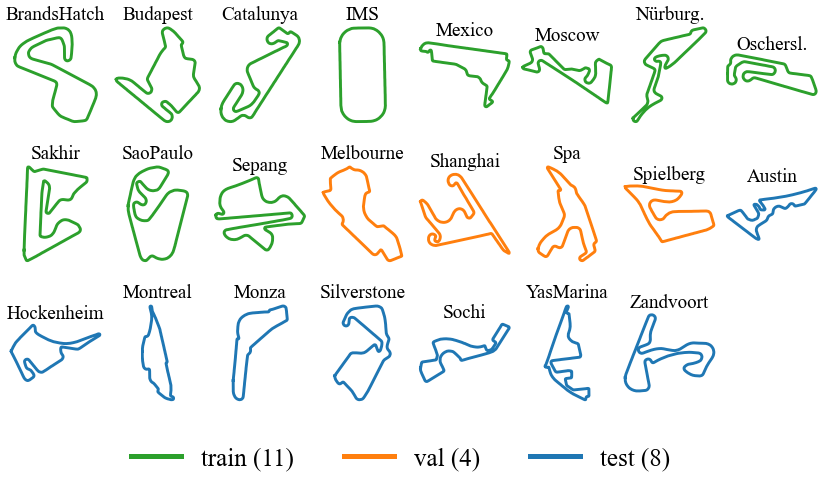
\includegraphics[width=0.93\columnwidth]{fig03_circuits}
\caption{The 23 extracted F1TENTH references, with color indicating the split.
Besides the three circuits that trained the naive-protocol bead (Yas Marina,
Montreal, Hockenheim), five more form the test set; none of them is used to
train, tune or select any controller.}
\label{fig:circuits}
\end{figure}

Each controller drives every test circuit five times (start perturbed by up to
$\pm5$~cm) and every test contour once, deterministically. Learned controllers have
five training seeds (three in the behaviour-cloning weight check). In
\emph{Track~A} each controller drives at its own pace; in \emph{Track~B} the
car is commanded no faster than $\vmatch=1.256$~m/s, the expert's mean speed on
the training circuits, and PP is tuned and RL--PP trained again at this speed;
Bead-PP runs at $\vmatch$. Counting training seeds separately, 60 controller
instances ran 8400 test episodes. Every metric was recomputed from the stored
trajectories, partly with independent code, and re-running 22 instances from their
saved checkpoints reproduced the trajectories bit for bit.

All distances are to \emph{polylines}, not to points. With $\mathcal{P}$ the set
of reference points, $P$ the polyline through them and $X$ the trajectory
polyline, the tracking error of sample $\mathbf{x}_t$ is
$e(\mathbf{x}_t)=\mathrm{dist}(\mathbf{x}_t,P)$, which yields the RMSE, the
largest error and the error's 95th percentile (P95); coverage counts the
reference points lying at most $\tau$ from the trajectory polyline,
\begin{equation}
\geom{\tau}=\frac{1}{|\mathcal{P}|}\sum_{\mathbf{p}\in\mathcal{P}}\one\big[\mathrm{dist}(\mathbf{p},X)\le\tau\big].
\label{eq:geom}
\end{equation}
Ordered coverage is the size of the biggest group of reference points reached
($\le\rho$) in path order, computed by dynamic programming; a run with ordered
coverage of at least 0.95 is completed. The same code scores every controller,
against the extracted reference and, for the circuits, against the true
centerline. Under a \emph{naive protocol} we also score a bead fitted to the
expert by regression, with its checkpoint chosen on Montreal, Yas Marina and
Hockenheim, an RL--PP agent trained on just one hand-drawn contour and run without
its normalization statistics, and PP with hand-set gains $(0.55~\mathrm{m},1.05)$
and $(a,b)=(0.35,0.25)$; these rows enter no comparison.

\parhead{Statistics.}Every comparison pairs the two controllers circuit by
circuit on the 8 test circuits, after averaging seeds and episodes. The main
evidence is the mean difference and its bootstrap interval at the 95\% level
(10\,000 resamples of circuits, and of seeds within learned controllers). With
$n=8$, an exact signed-rank Wilcoxon test cannot give $p<0.0078$, which requires all
circuits to agree, so only four primary RMSE comparisons are tested, with Holm
correction: (P1) Bead-DAgger versus Fixed PP at $\vmatch$; (P2) Bead-\dpo{}
versus Bead-DAgger; (P3) RL--PP joint versus Fixed PP; (P4) Bead-PP versus the
expert. They were declared before the final evaluation; a preliminary run of
Bead-PP and of the expert sweep had, however, touched the test circuits before
the settings were fixed (no setting was chosen from it). Other comparisons are
exploratory. Episodes are not pooled, since those on one circuit differ only by
the start perturbation.

%% ---------------- Table 4 (full width) ----------------------------------
\begin{table*}[t]
\caption{Accuracy against the extracted references on the eight unseen test
circuits, averaged over circuits with five episodes per circuit. Learned
controllers: average of five training seeds (three for $\lambda=10$), with the
seed range in brackets. Bold: most accurate entry of each column.}
\label{tab:main}
\centering
\resizebox{\textwidth}{!}{%
\begin{tabular}{@{}lcllcccccc@{}}
\toprule
Controller & $\geom{0.05}$ [\%] & $\geom{0.10}$ [\%] & RMSE [cm] & P95 [cm] & Max [cm] & Ordered [\%] & Completed [\%] & Time [s] & Speed [m/s]\\
\midrule
\multicolumn{10}{@{}l}{\emph{Bead plant (holonomic point mass, damping-limited)}}\\
Geometric expert~(3)                & 98.6 & \textbf{99.2} & 1.07 & 2.55 & 5.02 & \textbf{99.1} & 100 & 42.5 & 1.25\\
Bead-PP (PP law on bead)$^{\S}$     & \textbf{99.0} & \textbf{99.2} & \textbf{0.28} & 0.51 & \textbf{2.72} & \textbf{99.1} & 100 & 42.5 & 1.25\\
Bead-DAgger                         & 98.4 & 99.1 [99.1, 99.1] & 1.06 [1.05, 1.07] & 2.47 & 5.47 & \textbf{99.1} & 100 & 42.4 & 1.25\\
Bead-DAgger, Bead-PP teacher        & \textbf{99.0} & \textbf{99.2} [99.2, 99.2] & 0.42 [0.41, 0.43] & 0.83 & 3.19 & \textbf{99.1} & 100 & 42.8 & 1.24\\
Bead-\dpo{}                         & 96.6 & 99.1 [99.0, 99.1] & 1.77 [1.51, 2.14] & 3.56 & 7.39 & \textbf{99.1} & 100 & 42.2 & 1.25\\
Bead-\dpo{}, $\lambda=10$ (3 seeds) & 98.2 & 99.1 [99.1, 99.1] & 1.26 [1.22, 1.32] & 2.86 & 5.99 & \textbf{99.1} & 100 & 42.7 & 1.24\\
Bead-\dpo{}, prog.\ rew.            & 95.0 & 98.9 [98.8, 99.1] & 2.14 [1.75, 2.31] & 4.42 & 8.64 & \textbf{99.1} & 100 & 40.9 & 1.30\\
Bead-PPO (scratch)                  & 69.5 & 89.8 [82.6, 94.8] & 5.12 [4.25, 5.96] & 10.64 & 19.27 & 96.4 & 98 & 36.8 & 1.36\\
Bead-PPO (scratch), prog.\ rew.     & 59.0 & 83.1 [76.8, 86.0] & 6.49 [6.00, 7.73] & 13.63 & 22.29 & 95.9 & 74 & 37.0 & 1.38\\
Bead, naive protocol$^{*}$          & 77.0 & 93.9 & 4.38 & 9.26 & 16.30 & 98.9 & 100 & 42.5 & 1.23\\
\midrule
\multicolumn{10}{@{}l}{\emph{Bicycle plant, native speed profile (Track A)}}\\
Fixed PP (hand-set gains)           & 85.0 & 94.4 & 3.85 & 8.52 & 18.98 & 98.0 & 100 & 18.2 & 2.90\\
Fixed PP (tuned)                    & \textbf{99.0} & \textbf{99.2} & 0.34 & 0.57 & 3.26 & \textbf{99.1} & 100 & 18.5 & 2.87\\
Adaptive PP (hand-set)              & 24.8 & 33.7 & 10.12 & 22.97 & 32.55 & 40.8 & 0 & 8.0 & 2.89\\
Adaptive PP (tuned)                 & 98.9 & \textbf{99.2} & 0.42 & 0.69 & 3.83 & \textbf{99.1} & 100 & 18.5 & 2.87\\
Stanley (tuned)                     & 80.7 & 91.9 & 4.12 & 9.24 & 16.82 & 96.3 & 88 & 17.6 & 2.91\\
RL--PP (joint $\Ld,g$)~\cite{elgouhary2026} & 94.2 & 96.6 [91.5, 99.1] & 1.83 [1.27, 2.65] & 3.89 & 11.35 & 97.0 & 96 & 18.1 & 2.86\\
RL--PP ($\Ld$ only)                 & 97.7 & 99.0 [98.9, 99.1] & 1.57 [1.21, 2.16] & 3.23 & 10.14 & \textbf{99.1} & 100 & 18.7 & 2.86\\
RL--PP, naive protocol$^{\dagger}$  & 83.8 & 95.5 & 3.68 & 7.89 & 16.73 & 98.6 & 100 & 17.9 & 2.89\\
\midrule
\multicolumn{10}{@{}l}{\emph{Bicycle plant, speed capped at $\vmatch=1.256$~m/s (Track B)}}\\
Fixed PP (tuned)                    & \textbf{99.0} & \textbf{99.2} & 0.31 & 0.51 & 3.26 & \textbf{99.1} & 100 & 42.2 & 1.26\\
Adaptive PP (tuned)                 & 98.9 & \textbf{99.2} & 0.35 & \textbf{0.49} & 3.74 & \textbf{99.1} & 100 & 42.3 & 1.26\\
Stanley (tuned)                     & 77.6 & 88.7 & 3.56 & 8.65 & 16.87 & 92.6 & 88 & 39.3 & 1.26\\
RL--PP (joint $\Ld,g$)              & 93.6 & 95.6 [89.8, 99.0] & 2.40 [1.61, 4.10] & 4.75 & 15.19 & 96.0 & 94 & 41.3 & 1.26\\
\bottomrule
\end{tabular}}

\vspace{3pt}
\parbox{\textwidth}{\fontsize{7.5}{9}\selectfont
$^{*}$Naive protocol: actor regressed onto the expert and selected on three of
the eight test circuits (Yas Marina, Montreal, Hockenheim).\\
$^{\dagger}$Naive protocol: trained on just one hand-drawn contour; run on raw
observations. $^{\S}$The Fixed PP law executed on the bead at $\vmatch$.}
\end{table*}

%% =========================================================================
\section{Results and Discussion}

\subsection{Accuracy on held-out circuits}

Table~\ref{tab:main} gives the results against the extracted references.
\textbf{Bead-DAgger matches its expert} (1.06 versus 1.07~cm) with almost no
spread across seeds. All PPO-trained variants are less accurate:
Bead-\dpo{} reaches 1.77~cm (2.14~cm with the progress reward) while
scratch-trained Bead-PPO reaches 5.12~cm (6.49~cm), completing 98\% (74\%) of its test runs.
\textbf{Against these references, tuned Fixed PP is more accurate than every
learned bead controller}, including the one taught by PP
(Section~\ref{sec:law}): it reaches 0.34~cm at native speed and 0.31~cm at
$\vmatch$, and tuned Adaptive PP reaches 0.42~cm; RL--PP reaches 1.83~cm (joint)
and 1.57~cm ($\Ld$ only). Fig.~\ref{fig:accuracy} summarizes accuracy and spread
across seeds. Because both plants share the lap rule, $\geom{0.10}$ is equal for
every controller that completes its laps. Hand-set Adaptive PP completes no lap:
its lookahead of 0.8--1.6~m cuts corners by more than $\rho$. \textbf{Tuned
Stanley is less accurate than PP at the car's reference point}: 4.12~cm at
native and 3.56~cm at the matched speed, behind Fixed PP on every circuit
(3.25~cm [2.88, 3.54] at $\vmatch$; 2.67~cm against the true centerlines), and
it completes 88\% of its runs: at one Montreal hairpin its rear axle passes
about 20~cm from the path, beyond the lap counter's radius $\rho$, and the run
stops after 400 steps without progress. This follows from what each law
regulates: Stanley steers the front axle onto the path, so the rear axle cuts
corners by about $W^{2}/(2R)$ for a corner of radius $R$, whereas PP steers the
rear axle. At the front axle the order reverses (2.22~cm for Stanley, 4.83~cm
for Fixed PP at $\vmatch$). The car's position and all metrics refer to the rear
axle, so PP is the matching geometric law here, and our results on tuned
geometric control refer to PP.

%% ---------------- Fig. 3 -------------------------------------------------
\begin{figure}[t]
\centering
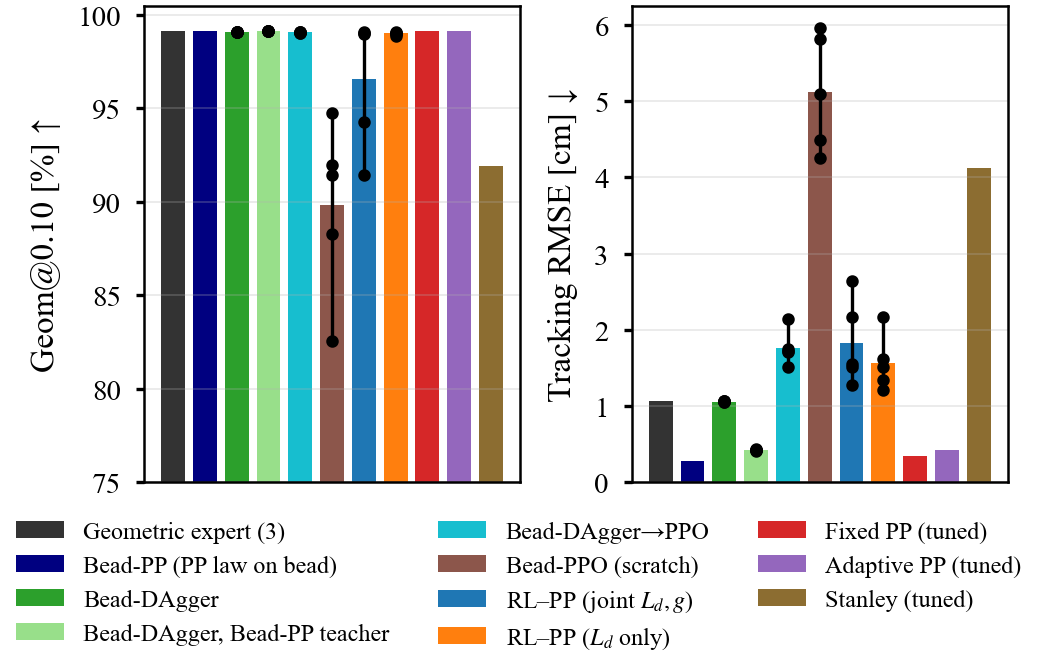
\includegraphics[width=\columnwidth]{fig04_accuracy}
\caption{Test-circuit averages. Left: $\geom{0.10}$ (higher is better).
Right: RMSE (lower is better). Dots mark the individual training seeds of
the learned controllers.}
\label{fig:accuracy}
\end{figure}

%% ---------------- Table 5 ------------------------------------------------
\begin{table}[t]
\caption{RMSE against the extracted references and RMSE, P95 and
$\geom{0.10}$ against the true F1TENTH centerlines (eight test circuits).}
\label{tab:true}
\centering
\resizebox{\columnwidth}{!}{%
\begin{tabular}{@{}lcccc@{}}
\toprule
 & Extracted & \multicolumn{3}{c}{True centerline}\\
\cmidrule(lr){2-2}\cmidrule(l){3-5}
Controller & RMSE & RMSE & P95 & G@0.10\\
 & [cm] & [cm] & [cm] & [\%]\\
\midrule
Geometric expert~(3)          & 1.07 & 1.60 & 3.16 & \textbf{99.2}\\
Bead-PP (PP law on bead)      & \textbf{0.28} & 1.24 & 1.99 & \textbf{99.2}\\
Bead-DAgger                   & 1.06 & 1.60 & 3.15 & 99.1\\
Bead-DAgger, Bead-PP teacher  & 0.42 & 1.24 & 2.03 & \textbf{99.2}\\
Bead-\dpo{}                   & 1.77 & 2.26 & 4.39 & 99.0\\
Bead-PPO (scratch)            & 5.12 & 5.49 & 11.38 & 88.8\\
Fixed PP (tuned)              & 0.34 & 1.25 & 2.04 & \textbf{99.2}\\
Fixed PP (tuned) @$\vmatch$   & 0.31 & \textbf{1.23} & \textbf{1.98} & \textbf{99.2}\\
Adaptive PP (tuned)           & 0.42 & 1.28 & 2.10 & \textbf{99.2}\\
Stanley (tuned)               & 4.12 & 4.44 & 9.81 & 91.6\\
Stanley (tuned) @$\vmatch$    & 3.56 & 3.90 & 9.24 & 88.2\\
RL--PP (joint $\Ld,g$)        & 1.83 & 2.22 & 4.47 & 96.5\\
\bottomrule
\end{tabular}}
\end{table}

Fig.~\ref{fig:laps} shows complete laps on three test circuits, and
Fig.~\ref{fig:cdf} the error distribution across the test circuits: under the
PP law, 99.8\% (Bead-PP), 99.8\% (Fixed PP) and 99.6\% (Adaptive PP) of all
samples lie closer than 3~cm to the reference, compared with 96.9\% for the
expert, 97.5\% for Bead-DAgger, 96.0\% for RL--PP, 92.7\% for Bead-\dpo{} and
60.4\% for Bead-PPO. The failures of the bead policies are visible in
Fig.~\ref{fig:zoom}: at the two Montreal corners with the largest Bead-\dpo{}
miss, that policy leaves by a small margin the almost common line of tuned
Fixed PP, RL--PP, the expert and Bead-DAgger, while scratch-trained Bead-PPO
drives inside the corner.

%% ---------------- Fig. 5 -------------------------------------------------
\begin{figure}[t]
\centering
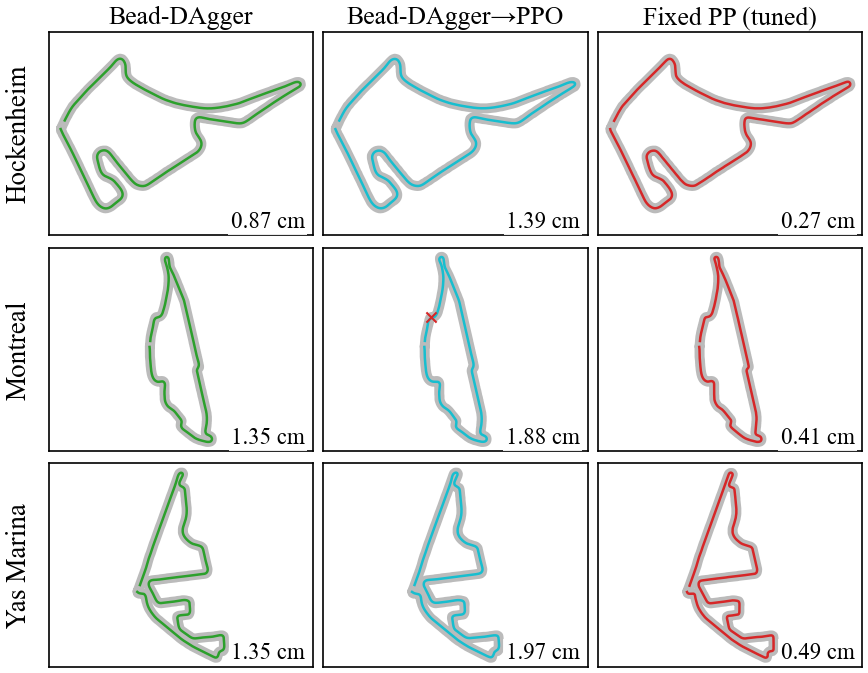
\includegraphics[width=\columnwidth]{fig05_laps}
\caption{Complete laps (first episode, seed 0) drawn over the grey reference on
three unseen circuits. A red cross marks a reference point missed by more than
0.10~m (the start/finish join is ignored); the number in each panel is the RMSE
of that lap.}
\label{fig:laps}
\end{figure}

%% ---------------- Fig. 6 -------------------------------------------------
\begin{figure}[t]
\centering
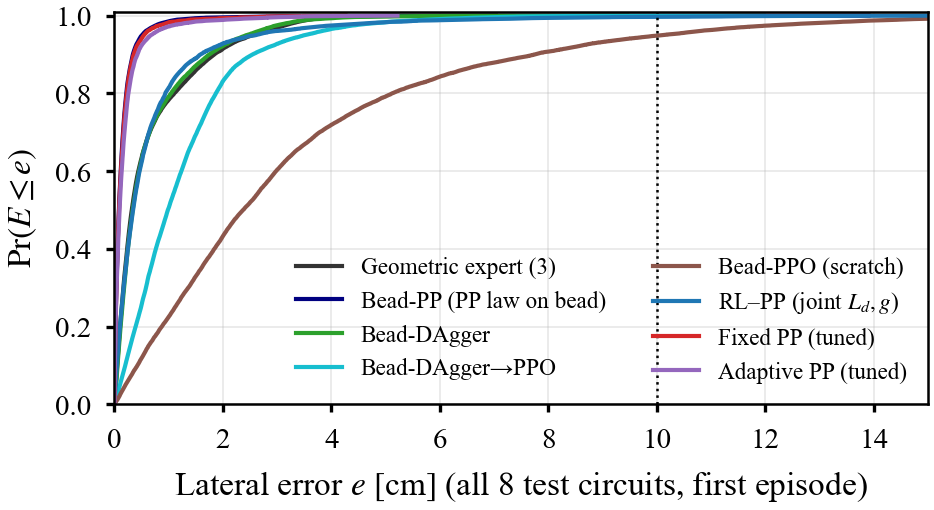
\includegraphics[width=\columnwidth]{fig06_cdf}
\caption{Fraction of trajectory samples whose distance to the extracted
reference stays below a threshold, with all eight test circuits taken together
(first episode; seed 0 for learned controllers). The dotted line is at
0.10~m.}
\label{fig:cdf}
\end{figure}

%% ---------------- Fig. 7 -------------------------------------------------
\begin{figure}[t]
\centering
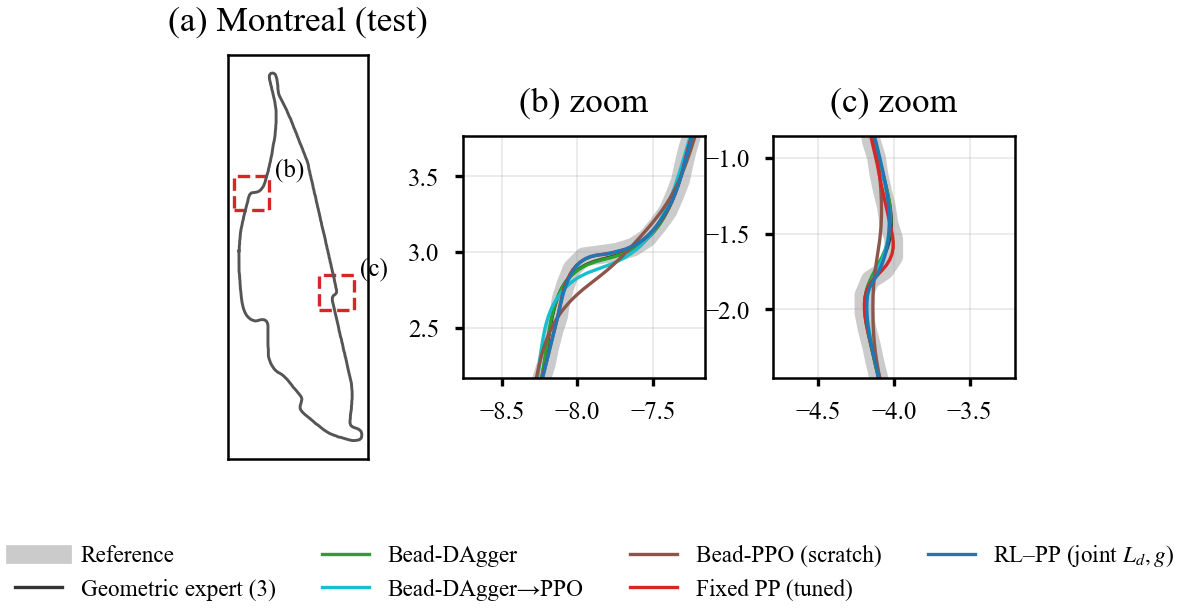
\includegraphics[width=\columnwidth]{fig07_montreal_zoom}
\caption{Close-up of the controllers on the unseen Montreal circuit (first
episode, seed 0). Both zoom windows are placed by the script at the two
reference points where Bead-\dpo{} strays furthest, leaving out the
start/finish area.}
\label{fig:zoom}
\end{figure}

\textbf{Measured against the true centerlines} (Table~\ref{tab:true}), every
error grows by the extraction error, and the differences between good
controllers shrink. The gap between Bead-DAgger and Fixed PP at $\vmatch$ falls
from 0.75 [0.62, 0.87]~cm to 0.36 [0.22, 0.51]~cm, and that between Bead-PP and
the expert from $-0.79$ to $-0.36$~cm. These gaps are of the size of the
extraction error itself (0.79--1.24~cm), but they keep their sign on all eight
circuits, all four primary intervals still exclude zero, and the ranking of all
controllers is nearly unchanged (rank correlation 0.993).

\subsection{Control law, vehicle and teacher}
\label{sec:law}

\textbf{The control law, not the vehicle, explains the gap.} On the bead at
$\vmatch$ the PP law reaches 0.28~cm, as accurate as on the equally fast car and below the expert on all eight circuits (P4). On the training circuits
its error depends on $\Ld$ in the same way on both plants, with the same optimum
(Fig.~\ref{fig:lookahead}, left), so the bead is not harder to steer accurately.
Aiming the expert further ahead does not help (Fig.~\ref{fig:lookahead}, right):
the best target is the next waypoint ($k=1$, 1.07~cm), or $k=2$ with the
nearest-point anchor (1.15~cm), and from $k=4$ on laps are no longer completed.
Unlike PP, the expert does not turn the offset of its target into a curvature
command.

\textbf{The teacher, more than the network, limited the imitation policy.}
Taught by Bead-PP instead of the expert, with the same
Algorithm~\ref{alg:dagger}, Bead-DAgger reaches 0.42~cm: $-0.64$~cm
[$-0.77$, $-0.48$] relative to the expert-taught policy, better on all eight
circuits. Against the extracted references it stays 0.15~cm [0.11, 0.18] behind
its teacher and 0.12~cm [0.08, 0.15] behind tuned PP on the equally fast car, on every circuit. Against the true centerlines both differences vanish:
0.00~cm [$-0.03$, 0.04] relative to its teacher and 0.01~cm [$-0.03$, 0.05]
relative to tuned PP (Table~\ref{tab:true}). The network can therefore represent
a controller as accurate as tuned PP on the real track, but by imitation it
approaches, and does not exceed, its teacher.

%% ---------------- Fig. 4 -------------------------------------------------
\begin{figure}[t]
\centering
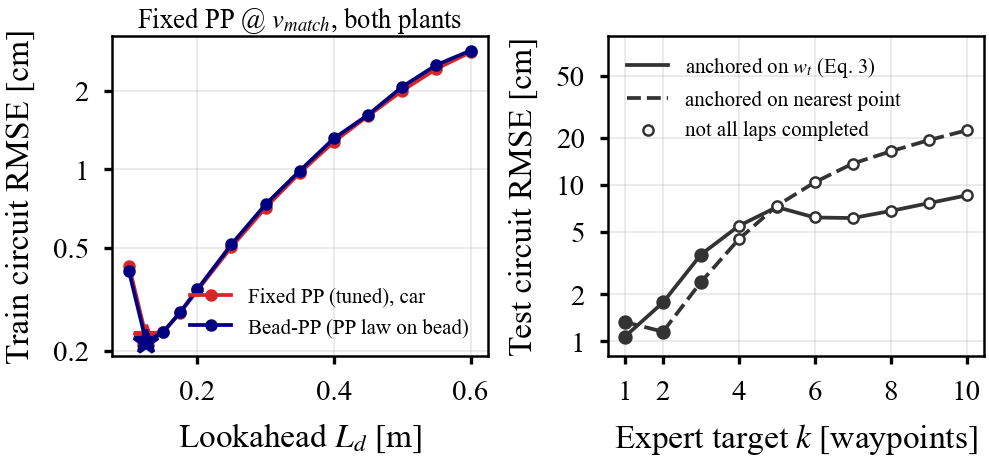
\includegraphics[width=\columnwidth]{fig08_lookahead}
\caption{Left: training-circuit RMSE of the same Fixed PP law on the car and on
the bead at $\vmatch$ versus $\Ld$ (best gain per $\Ld$; star: selected). Right:
test-circuit RMSE of the expert aiming $k$ waypoints ahead; open markers: not
every lap completed.}
\label{fig:lookahead}
\end{figure}

%% ---------------- Fig. 5 -------------------------------------------------
\begin{figure}[t]
\centering
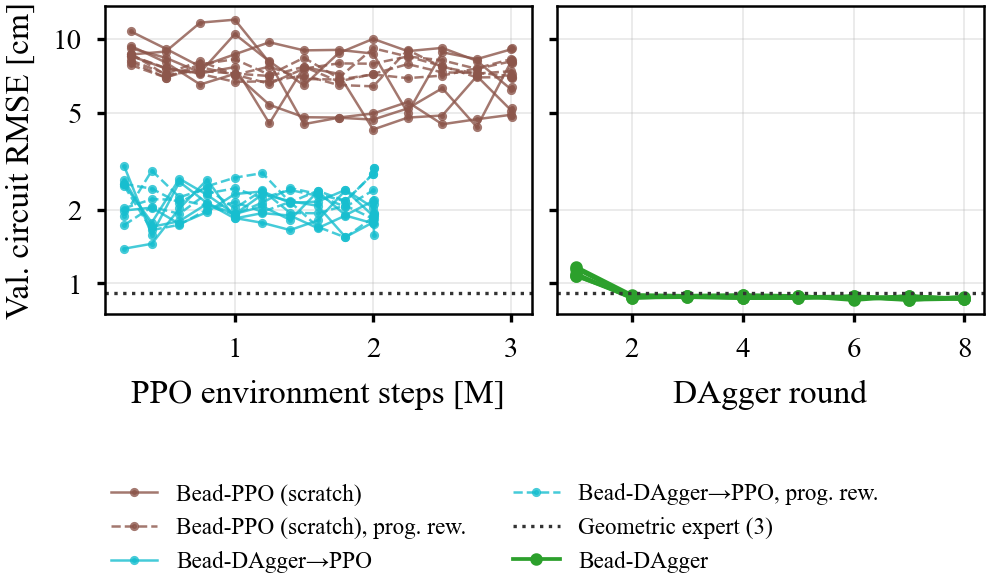
\includegraphics[width=\columnwidth]{fig09_training}
\caption{RMSE on the validation circuits as training proceeds (five seeds).
Left: PPO from random initial weights and PPO from the DAgger actor, with the
base (solid) and progress (dashed) reward. Right: the eight DAgger rounds
(expert teacher). Dotted: expert.}
\label{fig:training}
\end{figure}

%% ---------------- Fig. 10 ------------------------------------------------
\begin{figure}[t]
\centering
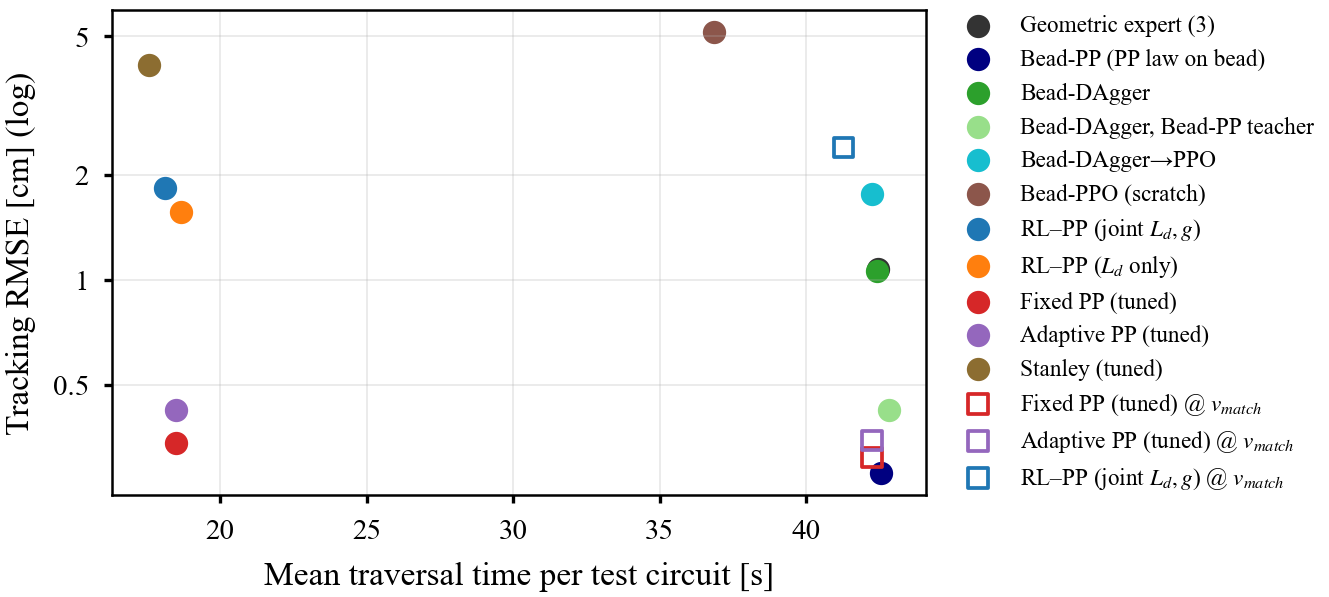
\includegraphics[width=\columnwidth]{fig10_laptime}
\caption{Accuracy against lap time on the test circuits. Solid circles: every
controller at its own speed (Track A). Hollow squares: the car's PP-family
controllers with their target speed limited to $\vmatch$ (Track B).}
\label{fig:laptime}
\end{figure}

\subsection{How PPO changes the bead policy}

PPO changes the actor, the critic and the action noise (unit tests; with the
actor frozen for the critic's warm-up the approximate KL divergence was exactly
zero); at the end of training the approximate KL per update is 0.010--0.031 and
the explained variance 0.86--0.98. PPO from scratch improves slowly and remains far
from the expert after $3\times10^{6}$ steps (Fig.~\ref{fig:training}).
Fine-tuning moves away from the DAgger policy despite the small initial noise,
the lower learning rate and the behaviour-cloning term, and raised the test RMSE
on all eight circuits for both rewards (P2). Ranked by base reward on these eight
circuits, the noise-free policies come out in the same order as by accuracy: the
expert collects 715, Bead-DAgger 715, Bead-\dpo{} 694 and Bead-PPO 534. PPO,
however, optimizes a stochastic policy, so each policy also drove the four
circuits of the validation split, both with and without Gaussian noise on its
actions (three
noise seeds, five training seeds). With the base reward, deterministic
Bead-DAgger earns 747 (RMSE 0.86~cm) and, with the initial fine-tuning noise,
749 (1.05~cm); the fine-tuned policy obtains 729 under its own noise
($\sigma\approx0.13$) and 729 noise-free (1.56~cm). With the progress reward the
returns are 838 and 829 before and 804 and 811 after fine-tuning (1.84~cm
deterministic). Fine-tuning thus lowered the return of the stochastic policy it
optimizes, under either reward, so the drop in accuracy cannot be explained by
training a noisy policy and testing a noise-free one. With the progress reward
the bead became faster and less accurate. A check of the behaviour-cloning
weight (seeds 0--2, base reward, selection on validation only) gave mean
validation RMSEs of 2.18, 1.57 and 1.09~cm for $\lambda=0.1$, 1 and 10, against
0.86~cm for the DAgger policy. With the selected $\lambda=10$, the fine-tuned
policy reaches 1.26~cm on the eight test circuits: less degraded than with
$\lambda=1$, but still 0.20~cm [0.15, 0.26] behind its starting point. Which
factor---the critic, the mix of long circuits and short
contours, the step size or the budget---causes the degradation was not isolated:
\textbf{with our PPO budget and settings, PPO did not improve the imitation
policy}.

\subsection{Naive protocol, speed and contours}

On its own training circuits (Hockenheim, Montreal, Yas Marina) the naive bead
reaches 2.45--4.05~cm, against 3.62--5.54~cm for PP with hand-set gains and
3.72--4.58~cm for naive RL--PP, so on each circuit direct actuation appears the
most precise of the three (Table~\ref{tab:naive}). However, tuned PP reaches 0.27--0.50~cm on the same circuits and the
expert that the naive bead imitates 0.94--1.36~cm. Over all eight test circuits,
Fixed PP with hand-set gains reaches 3.85~cm and naive RL--PP 3.68~cm. The naive bead averages 3.32~cm on
its training circuits but 5.02~cm on the five unseen ones: untuned baselines
reverse the ranking, and leakage inflates the learned controller.

%% ---------------- Table 6 ------------------------------------------------
\begin{table}[t]
\caption{Scores on the three circuits that trained the naive-protocol bead, as
$\geom{0.10}$ [\%] and RMSE [cm]; bold marks the best entry per column.}
\label{tab:naive}
\centering
\resizebox{\columnwidth}{!}{%
\begin{tabular}{@{}lcccccc@{}}
\toprule
 & \multicolumn{2}{c}{Hockenheim} & \multicolumn{2}{c}{Montreal} & \multicolumn{2}{c}{Yas Marina}\\
\cmidrule(lr){2-3}\cmidrule(lr){4-5}\cmidrule(l){6-7}
Controller & G@0.10 & RMSE & G@0.10 & RMSE & G@0.10 & RMSE\\
\midrule
Geometric expert~(3)          & \textbf{99.1} & 0.94 & \textbf{99.3} & 1.24 & \textbf{99.1} & 1.36\\
Bead-DAgger                   & \textbf{99.1} & 0.87 & \textbf{99.3} & 1.35 & \textbf{99.1} & 1.40\\
Bead, naive protocol$^{*}$    & \textbf{99.1} & 2.45 & 96.1 & 3.45 & 95.6 & 4.05\\
Fixed PP (hand-set gains)     & 95.7 & 3.62 & 90.8 & 5.54 & 89.8 & 5.17\\
Fixed PP (tuned)              & \textbf{99.1} & \textbf{0.27} & \textbf{99.3} & \textbf{0.41} & \textbf{99.1} & \textbf{0.50}\\
RL--PP (joint $\Ld,g$)~\cite{elgouhary2026} & 98.7 & 1.64 & 99.0 & 1.60 & 95.5 & 2.40\\
RL--PP, naive protocol$^{\dagger}$ & 96.1 & 3.72 & 94.2 & 4.40 & 91.9 & 4.58\\
\bottomrule
\end{tabular}}
\end{table}

Driving at its own pace, the bead needs about 2.3 times the car's lap time
(42.5 versus 18.5~s, Fig.~\ref{fig:laptime}), as friction caps its speed at
roughly 1.3~m/s, whereas the car's speed profile peaks at 5~m/s on straight
segments. At $\vmatch$ the car's lap time nearly equals the bead's (42.2 versus 42.5~s) and its
error drops slightly, to 0.31~cm with re-tuned Fixed PP and 0.35~cm with Adaptive
PP, while retrained RL--PP reaches 2.40~cm; tuned PP is still the more accurate
(P1).

%% ---------------- Table 7 ------------------------------------------------
\begin{table}[t]
\caption{Eight test circuits at $\vmatch$ on the dynamic single-track car:
(a) tyres only, (b) tyres and steering-rate limit. Settings: $(\Ld,g)$ or
$(k,k_s)$. RMSE in cm against the extracted reference (Extr.) and the true
centerline (True); Laps: \% completed.}
\label{tab:dynamic}
\centering
\resizebox{\columnwidth}{!}{%
\begin{tabular}{@{}lcccc|cccc@{}}
\toprule
 & \multicolumn{4}{c|}{(a) Tyres only} & \multicolumn{4}{c}{(b) Tyres + rate limit}\\
Controller & Settings & Extr. & True & Laps & Settings & Extr. & True & Laps\\
\midrule
Fixed PP, re-tuned            & (0.175, 2.5) & 1.83 & 2.31 & 100 & (0.45, 1.6) & 3.09 & 3.53 & 100\\
Fixed PP, re-tuned, $g\le1.4$ & (0.2, 1.4)   & 1.91 & 2.30 & 100 & (0.4, 1.4)  & 3.23 & 3.59 & 88\\
Stanley, re-tuned             & (8, 0.25)    & 2.66 & 3.11 & 100 & (4, 0.05)   & 3.58 & 3.83 & 88\\
RL--PP, retrained             & --           & 5.26 & 5.38 & 82  & --          & 6.73 & 6.82 & 50\\
\midrule
Fixed PP, unchanged           & --           & 3.95 & 4.11 & 88  & --          & 34.84 & 34.77 & 0\\
Stanley, unchanged            & --           & 2.80 & 3.23 & 100 & --          & 28.38 & 28.47 & 0\\
RL--PP, unchanged             & --           & 5.68 & 5.71 & 73  & --          & 23.52 & 23.39 & 2\\
\bottomrule
\end{tabular}}
\end{table}

\parhead{Dynamic vehicle model.}To check whether the kinematic car flatters PP,
the car controllers were also run at $\vmatch$ on the dynamic single-track model
with linear tyres of F1TENTH Gym~\cite{okelly2020f1tenth} (its mass, inertia,
axle distances, cornering stiffnesses and switch to kinematics below 0.5~m/s;
position at the rear axle; steering limit kept at $\pm1.10$~rad, as arena
hairpins need about 1~rad), (a) with the tyres alone and (b) also with its
steering-rate limit of 3.2~rad/s, a full-scale actuator value applied to shrunk
circuits. Fixed PP and Stanley were re-tuned on each model with the same grids,
references and score as before, and RL--PP was retrained
(Table~\ref{tab:dynamic}). \textbf{Gains tuned on the kinematic car do not
transfer}: unchanged, Fixed PP reaches 3.95~cm in (a) and completes no lap in
(b). \textbf{Re-tuned, Fixed PP is again the most accurate car controller}, at
1.83~cm in (a) and 3.09~cm in (b), about six and ten times its kinematic error,
and it beats retrained RL--PP on all eight circuits (differences $-3.42$~cm
[$-4.96$, $-2.22$] and $-3.64$~cm [$-5.90$, $-2.06$]). The lead over Stanley is
clear with tyres only, $-0.82$~cm [$-1.44$, $-0.10$] and better on 7 of 8
circuits, and unclear with the rate limit, $-0.49$~cm [$-1.22$, 0.18]. These
results use an extended gain range ($g\le6$ in (a), $g\le2.5$ in (b)): on the
shared grid the selected gain sits on the top edge ($g=1.4$), against our
inside-the-range rule, and in (b) no setting completes every training lap. The
extended optima lie inside the range and complete every test lap; the
shared-grid result (Table~\ref{tab:dynamic}) is equal within the intervals. In
(b) no Stanley setting completes every training lap, so the best-scoring one
was used, and it fails on Yas Marina. The bead has no tyres, so the comparison
with it holds only at equal model fidelity: re-tuned PP on the tyre car
(1.83~cm) is less accurate than Bead-DAgger on the tyre-free bead (1.06~cm).

%% ---------------- Fig. 11 ------------------------------------------------
\begin{figure}[t]
\centering
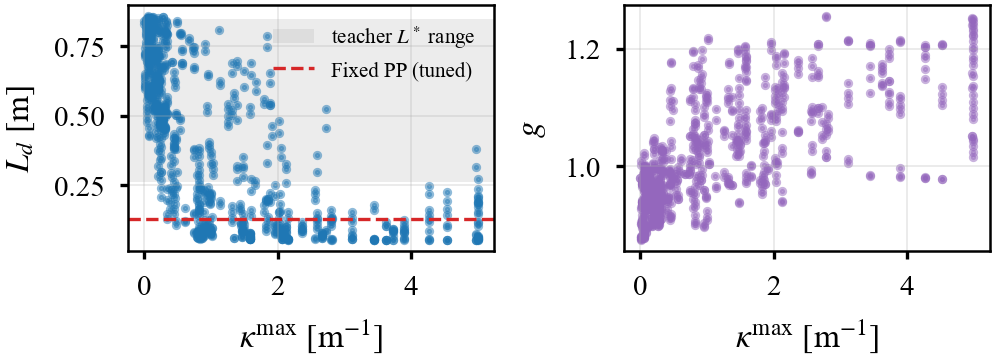
\includegraphics[width=\columnwidth]{fig11_rlpp_schedule}
\caption{Lookahead and gain chosen by the joint RL--PP agent (seed 0) while
driving the unseen Montreal circuit: $\Ld$ and $g$ versus previewed curvature.
Shaded: teacher's $L^{*}$ range; dashed: tuned Fixed PP.}
\label{fig:schedule}
\end{figure}

The synthetic test set of 100 contours is covered by Table~\ref{tab:synth}. The ranking
of the circuits carries over: Bead-PP and tuned Fixed PP are the most accurate,
Bead-DAgger matches the expert, and the PPO-trained beads and naive-protocol
checkpoints are less accurate. Coverage saturates: the good controllers all
reach the largest $\geom{0.10}$ that the lap rule allows (99.1\% on closed
shapes, 98.6--98.7\% on open curves), so among them only RMSE separates the
controllers.

%% ---------------- Table 8 ------------------------------------------------
\begin{table}[t]
\caption{Accuracy on the synthetic test set of 100 contours; $\geom{0.10}$ is
given as average $\pm$ standard deviation over the contours, and the best entry
of each set is bold. $^{*}$,~$^{\dagger}$: naive protocol; $^{\S}$: Fixed PP
law on the bead.}
\label{tab:synth}
\centering
\resizebox{\columnwidth}{!}{%
\begin{tabular}{@{}lcccc@{}}
\toprule
Set / Controller & $\geom{0.10}$ [\%] & RMSE [cm] & Ordered [\%] & Time [s]\\
\midrule
\multicolumn{5}{@{}l}{\emph{Closed shapes (50)}}\\
Geometric expert~(3)                  & \textbf{99.1} $\pm$ 0.3 & 1.12 & \textbf{99.1} & 24.4\\
Bead-PP (PP law on bead)$^{\S}$       & \textbf{99.1} $\pm$ 0.4 & 0.69 & \textbf{99.1} & 24.8\\
Bead-DAgger                           & \textbf{99.1} $\pm$ 0.4 & 1.17 & \textbf{99.1} & 24.4\\
Bead-\dpo{}                           & \textbf{99.1} $\pm$ 0.4 & 1.56 & \textbf{99.1} & 24.4\\
Bead-PPO (scratch)                    & 98.2 $\pm$ 1.1 & 2.94 & \textbf{99.1} & 22.0\\
Fixed PP (tuned)                      & \textbf{99.1} $\pm$ 0.3 & \textbf{0.63} & \textbf{99.1} & 10.8\\
RL--PP (joint $\Ld,g$)~\cite{elgouhary2026} & 98.8 $\pm$ 0.5 & 1.46 & \textbf{99.1} & 10.8\\
Bead, naive protocol$^{*}$            & 96.2 $\pm$ 2.8 & 3.90 & 99.0 & 25.1\\
RL--PP, naive protocol$^{\dagger}$    & 97.8 $\pm$ 1.4 & 2.35 & 99.0 & 10.7\\
\midrule
\multicolumn{5}{@{}l}{\emph{Open curves (50)}}\\
Geometric expert~(3)                  & 98.6 $\pm$ 0.1 & 1.06 & \textbf{99.1} & 15.5\\
Bead-PP (PP law on bead)$^{\S}$       & 98.6 $\pm$ 0.1 & 0.71 & \textbf{99.1} & 15.7\\
Bead-DAgger                           & 98.6 $\pm$ 0.1 & 1.09 & \textbf{99.1} & 15.5\\
Bead-\dpo{}                           & 98.6 $\pm$ 0.1 & 1.46 & \textbf{99.1} & 15.4\\
Bead-PPO (scratch)                    & 98.4 $\pm$ 0.7 & 2.42 & \textbf{99.1} & 13.8\\
Fixed PP (tuned)                      & \textbf{98.7} $\pm$ 0.1 & \textbf{0.69} & \textbf{99.1} & 8.5\\
RL--PP (joint $\Ld,g$)~\cite{elgouhary2026} & \textbf{98.7} $\pm$ 0.1 & 1.19 & \textbf{99.1} & 8.5\\
Bead, naive protocol$^{*}$            & 98.4 $\pm$ 0.6 & 2.58 & \textbf{99.1} & 15.9\\
RL--PP, naive protocol$^{\dagger}$    & 98.5 $\pm$ 0.4 & 1.65 & \textbf{99.1} & 8.5\\
\bottomrule
\end{tabular}}
\end{table}

\subsection{The learned PP schedule}

The RL--PP agent shortens its lookahead before corners (correlation $-0.68$ with
the previewed curvature) and raises its gain in corners (correlation $+0.70$), as
described in~\cite{elgouhary2026} (Fig.~\ref{fig:schedule}). Its median
lookahead over all test circuits and seeds is, however, 0.44~m, with 57\% of its
steps inside the teacher's band $[0.26,0.85]$~m, far above the 0.125~m selected
for Fixed PP: its reward pulls it toward a teacher that favours long lookaheads,
which explains why it is less accurate than tuned constant PP (P3). The
$\Ld$-only agent shows a small but uncertain advantage over the joint agent: it
is better on 7 of 8 circuits, but the mean difference 0.26~cm has the interval
[$-0.30$, 0.87]. We did not redesign the teacher, which would tune the method
of~\cite{elgouhary2026} beyond adapting it.

\subsection{Statistical evidence}

In all four primary comparisons (Table~\ref{tab:paired}) the same controller is
better on all eight circuits, so $p=0.0078$, which remains below 0.05 after Holm correction ($p=0.031$).
With eight circuits this only says that all circuits agree; effect sizes are
given by the intervals, which describe variation over these circuits and seeds,
not over other simulators, scales or vehicles.

%% ---------------- Table 9 (full width) ----------------------------------
\begin{table*}[t]
\caption{Pairwise RMSE differences $A-B$ in cm across all eight test circuits
(negative favours $A$; 95\% bootstrap interval over circuits and training
seeds; exact Wilcoxon test). Left: against the extracted references. Right: the
same comparison against the true F1TENTH centerlines, recomputed from the stored
trajectories.}
\label{tab:paired}
\centering
\resizebox{\textwidth}{!}{%
\begin{tabular}{@{}lrlcccrl@{}}
\toprule
 & \multicolumn{5}{c}{Extracted reference} & \multicolumn{2}{c}{True centerline}\\
\cmidrule(lr){2-6}\cmidrule(l){7-8}
$A$ vs $B$ & Diff. & 95\% CI & Better & $p$ & Holm & Diff. & 95\% CI\\
\midrule
\multicolumn{8}{@{}l}{\emph{Primary (Holm over these four)}}\\
DAgger vs Fixed PP @$\vmatch$ & $+0.75$ & [$+0.62$, $+0.87$] & 0/8 & 0.0078 & 0.031 & $+0.36$ & [$+0.22$, $+0.51$]\\
\dpo{} vs DAgger               & $+0.71$ & [$+0.53$, $+0.93$] & 0/8 & 0.0078 & 0.031 & $+0.66$ & [$+0.39$, $+0.97$]\\
RL--PP joint vs Fixed PP       & $+1.49$ & [$+1.06$, $+2.02$] & 0/8 & 0.0078 & 0.031 & $+0.97$ & [$+0.55$, $+1.49$]\\
Bead-PP vs Expert              & $-0.79$ & [$-0.92$, $-0.64$] & 8/8 & 0.0078 & 0.031 & $-0.36$ & [$-0.49$, $-0.23$]\\
\midrule
\multicolumn{8}{@{}l}{\emph{Exploratory (no correction)}}\\
DAgger vs Expert                                 & $-0.01$ & [$-0.06$, $+0.04$] & 5/8 & 0.8438 & -- & $-0.00$ & [$-0.04$, $+0.04$]\\
DAgger (Bead-PP teacher) vs DAgger               & $-0.64$ & [$-0.77$, $-0.48$] & 8/8 & 0.0078 & -- & $-0.36$ & [$-0.52$, $-0.19$]\\
DAgger (Bead-PP teacher) vs Bead-PP              & $+0.15$ & [$+0.11$, $+0.18$] & 0/8 & 0.0078 & -- & $+0.00$ & [$-0.03$, $+0.04$]\\
DAgger (Bead-PP teacher) vs Fixed PP @$\vmatch$  & $+0.12$ & [$+0.08$, $+0.15$] & 0/8 & 0.0078 & -- & $+0.01$ & [$-0.03$, $+0.05$]\\
\dpo{} ($\lambda=10$) vs DAgger                   & $+0.20$ & [$+0.15$, $+0.26$] & 0/8 & 0.0078 & -- & $+0.13$ & [$+0.05$, $+0.21$]\\
\dpo{} ($\lambda=10$) vs \dpo{}                   & $-0.50$ & [$-0.75$, $-0.31$] & 8/8 & 0.0078 & -- & $-0.53$ & [$-0.84$, $-0.24$]\\
\dpo{} vs Expert                                  & $+0.69$ & [$+0.53$, $+0.94$] & 0/8 & 0.0078 & -- & $+0.66$ & [$+0.41$, $+0.99$]\\
PPO (scratch) vs \dpo{}                           & $+3.36$ & [$+2.35$, $+4.92$] & 0/8 & 0.0078 & -- & $+3.23$ & [$+2.23$, $+4.83$]\\
\dpo{} (prog.) vs \dpo{}                          & $+0.37$ & [$+0.08$, $+0.64$] & 0/8 & 0.0078 & -- & $+0.30$ & [$-0.05$, $+0.66$]\\
PPO (scratch, prog.) vs PPO (scratch)             & $+1.37$ & [$+0.19$, $+2.33$] & 0/8 & 0.0078 & -- & $+1.38$ & [$+0.17$, $+2.42$]\\
Bead-PP vs Fixed PP @$\vmatch$                    & $-0.03$ & [$-0.08$, $+0.03$] & 5/8 & 0.5469 & -- & $+0.01$ & [$-0.01$, $+0.02$]\\
Fixed PP @$\vmatch$ vs Expert                     & $-0.76$ & [$-0.86$, $-0.66$] & 8/8 & 0.0078 & -- & $-0.36$ & [$-0.49$, $-0.25$]\\
RL--PP joint vs RL--PP $\Ld$                      & $+0.26$ & [$-0.30$, $+0.87$] & 1/8 & 0.0234 & -- & $+0.27$ & [$-0.24$, $+0.82$]\\
Adaptive PP vs Fixed PP                           & $+0.08$ & [$+0.06$, $+0.11$] & 0/8 & 0.0078 & -- & $+0.03$ & [$+0.02$, $+0.05$]\\
Stanley vs Fixed PP                               & $+3.78$ & [$+3.45$, $+4.05$] & 0/8 & 0.0078 & -- & $+3.19$ & [$+2.88$, $+3.44$]\\
Stanley @$\vmatch$ vs Fixed PP @$\vmatch$         & $+3.25$ & [$+2.88$, $+3.54$] & 0/8 & 0.0078 & -- & $+2.67$ & [$+2.31$, $+2.97$]\\
\bottomrule
\end{tabular}}
\end{table*}

\subsection{Threats to validity}

\begin{itemize}
\item \textbf{Extraction error and spacing.} Differences below about 1~cm are
  within the extraction error (Table~\ref{tab:true}). The Austin test reference does not close exactly
  (Table~\ref{tab:spacing}); closing it changes RMSE by at most 0.012~cm and no
  lap outcome. Waypoints are 11.1--23.5~cm apart, which may disadvantage the
  expert, whose target is the next waypoint, whereas PP interpolates its
  lookahead point.
\item \textbf{PPO budget and settings.} 2--$3\times10^{6}$ steps per run; of the
  fine-tuning settings only the behaviour-cloning weight was varied
  ($\lambda\in\{0.1,1,10\}$, three seeds), while initial noise, learning rate
  and critic warm-up were fixed. Our results show that PPO did not improve the
  policy under these settings, not that it cannot.
\item \textbf{RL--PP adaptation.} Scale, ranges, teacher, reward weights and
  budget differ from~\cite{elgouhary2026} (Table~\ref{tab:rlpp}); results
  characterize our adaptation.
\item \textbf{Plants and scale.} Bead-PP controls for the plant for one law and
  one speed; the main comparison uses a kinematic car (dynamic model:
  Table~\ref{tab:dynamic}); tracks are shrunk 4.3--9.8$\times$.
\item \textbf{Exposure and scope.} Three test circuits were known when the
  reward was designed, and a preliminary run touched the test circuits
  (Section~4.1); five seeds; only 50 of the 150 test contours in each synthetic set;
  simulation only. Not yet tested: sensor noise and true-scale circuits with
  real steering limits.
\end{itemize}

%% =========================================================================
\section{Conclusion}

Under shared paths, measures and lap rule, we compared learning that replaces a
geometric tracking law with learning integrated into it, on held-out circuits.
The DAgger-trained bead matched its hand-written teacher; taught by the PP law,
it came within 0.15~cm of that law on the extracted references and matched it,
and tuned PP on the car, against the true centerlines, so the teacher, more than
the network, limited imitation. With our PPO budget and settings, PPO did not
improve the imitation policy, whether started from scratch or fine-tuned, with either reward
or any behaviour-cloning weight tried. A tuned PP law was more accurate than
every learned controller that did not imitate it, on the kinematic car and on the bead,
so the gap comes from the control law rather than the vehicle; it shrinks to
0.36~cm against the true centerlines but keeps its sign on every circuit. Our
RL-tuned PP reproduced the qualitative schedule of~\cite{elgouhary2026} but
followed a teacher with long lookaheads. A naive protocol would have reversed
these conclusions. A well-tuned PP law is thus a strong baseline (tuned Stanley,
which regulates the front axle, less so). On a dynamic car it stays the most
accurate car controller only after re-tuning, with a smaller margin, so
baselines should be tuned on the vehicle model used for comparison. Integrating
learning with PP, for example as a learned residual, is a more promising
direction than replacing it, together with hardware tests.

%% =========================================================================
\section*{Declarations}

\subsection*{Conflict of Interest}
The authors have no financial or personal interests to declare that are
relevant to this work.

\subsection*{Funding}
Not applicable.

\subsection*{Authors' Contributions}
All authors contributed to the development and preparation of this research. Dileep and Sanjay contributed to the conceptualization, methodology, implementation, experimentation, and manuscript preparation. Atin and Piyush contributed to the technical guidance, review, and refinement of the manuscript.

\subsection*{Data Availability}
The code, data split, trained checkpoints, raw test trajectories and the
scripts that generate every table and number of this paper are available at
\url{https://github.com/sanjayvarma06/Bead-Simulation-using-RL}.

\subsection*{Code Availability}
The source code and scripts used in this study are available at:
\url{https://github.com/sanjayvarma06/Bead-Simulation-using-RL}.

The F1TENTH centerlines come from
the public F1TENTH racetrack collection.

%% =========================================================================
\renewcommand{\refname}{References}
{\fontsize{9}{10.8}\selectfont
\begin{thebibliography}{99}
\setlength{\itemsep}{1pt}

\bibitem{okelly2020f1tenth}
M.~O'Kelly, H.~Zheng, D.~Karthik, and R.~Mangharam, ``F1TENTH: An
open-source evaluation environment for continuous control and reinforcement
learning,'' \emph{Proc.\ of the NeurIPS 2019 Competition and Demonstration
Track}, PMLR, vol.~123, pp.~77-89, 2020.

\bibitem{coulter1992}
R.~C. Coulter, ``Implementation of the pure pursuit path tracking algorithm,''
Technical Report CMU-RI-TR-92-01, Robotics Institute, Carnegie Mellon
University, 1992.

\bibitem{snider2009}
J.~M. Snider, ``Automatic steering methods for autonomous automobile path
tracking,'' Technical Report CMU-RI-TR-09-08, Robotics Institute, Carnegie
Mellon University, 2009.

\bibitem{elgouhary2026}
M.~Elgouhary and A.~S. El-Wakeel, ``Learning to tune pure pursuit in
autonomous racing: Joint lookahead and steering-gain control with PPO,''
\emph{arXiv preprint} arXiv:2602.18386, 2026.

\bibitem{schulman2017ppo}
J.~Schulman, F.~Wolski, P.~Dhariwal, A.~Radford, and O.~Klimov, ``Proximal
policy optimization algorithms,'' \emph{arXiv preprint} arXiv:1707.06347, 2017.

\bibitem{ross2011dagger}
S.~Ross, G.~J. Gordon, and J.~A. Bagnell, ``A reduction of imitation learning
and structured prediction to no-regret online learning,'' \emph{Proc.\ of the
14th International Conference on Artificial Intelligence and Statistics
(AISTATS)}, pp.~627-635, 2011.

\bibitem{hoffmann2007}
G.~M. Hoffmann, C.~J. Tomlin, M.~Montemerlo, and S.~Thrun, ``Autonomous
automobile trajectory tracking for off-road driving: Controller design,
experimental validation and racing,'' \emph{Proc.\ of the American Control
Conference}, pp.~2296-2301, 2007.

\bibitem{rajamani2012}
R.~Rajamani, \emph{Vehicle Dynamics and Control}, 2nd ed., Springer, New York,
2012.

\bibitem{kong2015}
J.~Kong, M.~Pfeiffer, G.~Schildbach, and F.~Borrelli, ``Kinematic and dynamic
vehicle models for autonomous driving control design,'' \emph{Proc.\ of the
IEEE Intelligent Vehicles Symposium}, pp.~1094-1099, 2015.

\bibitem{heilmeier2020}
A.~Heilmeier, A.~Wischnewski, L.~Hermansdorfer, J.~Betz, M.~Lienkamp, and
B.~Lohmann, ``Minimum curvature trajectory planning and control for an
autonomous race car,'' \emph{Vehicle System Dynamics}, vol.~58, no.~10,
pp.~1497-1527, 2020.

\bibitem{betz2022}
J.~Betz, H.~Zheng, A.~Liniger, U.~Rosolia, P.~Karle, M.~Behl, V.~Krovi, and
R.~Mangharam, ``Autonomous vehicles on the edge: A survey on autonomous vehicle
racing,'' \emph{IEEE Open Journal of Intelligent Transportation Systems},
vol.~3, pp.~458-488, 2022.

\bibitem{kiran2022}
B.~R. Kiran, I.~Sobh, V.~Talpaert, P.~Mannion, A.~A. Al~Sallab, S.~Yogamani,
and P.~P\'erez, ``Deep reinforcement learning for autonomous driving: A
survey,'' \emph{IEEE Transactions on Intelligent Transportation Systems},
vol.~23, no.~6, pp.~4909-4926, 2022.

\bibitem{kober2013}
J.~Kober, J.~A. Bagnell, and J.~Peters, ``Reinforcement learning in robotics:
A survey,'' \emph{International Journal of Robotics Research}, vol.~32,
no.~11, pp.~1238-1274, 2013.

\bibitem{schulman2016gae}
J.~Schulman, P.~Moritz, S.~Levine, M.~Jordan, and P.~Abbeel,
``High-dimensional continuous control using generalized advantage
estimation,'' \emph{Proc.\ of the International Conference on Learning
Representations (ICLR)}, 2016.

\bibitem{andrychowicz2021}
M.~Andrychowicz, A.~Raichuk, P.~Sta\'nczyk, M.~Orsini, S.~Girgin, R.~Marinier,
L.~Hussenot, M.~Geist, O.~Pietquin, M.~Michalski, S.~Gelly, and O.~Bachem,
``What matters in on-policy reinforcement learning? A large-scale empirical
study,'' \emph{Proc.\ of the International Conference on Learning
Representations (ICLR)}, 2021.

\bibitem{haarnoja2018}
T.~Haarnoja, A.~Zhou, P.~Abbeel, and S.~Levine, ``Soft actor-critic:
Off-policy maximum entropy deep reinforcement learning with a stochastic
actor,'' \emph{Proc.\ of the 35th International Conference on Machine Learning
(ICML)}, pp.~1861-1870, 2018.

\bibitem{evans2023}
B.~D. Evans, H.~W. Jordaan, and H.~A. Engelbrecht, ``Comparing deep
reinforcement learning architectures for autonomous racing,'' \emph{Machine
Learning with Applications}, vol.~14, 100496, 2023.

\bibitem{pomerleau1989}
D.~A. Pomerleau, ``ALVINN: An autonomous land vehicle in a neural network,''
\emph{Advances in Neural Information Processing Systems 1}, pp.~305-313, 1989.

\bibitem{otsu1979}
N.~Otsu, ``A threshold selection method from gray-level histograms,''
\emph{IEEE Transactions on Systems, Man, and Cybernetics}, vol.~9, no.~1,
pp.~62-66, 1979.

\bibitem{zhang1984}
T.~Y. Zhang and C.~Y. Suen, ``A fast parallel algorithm for thinning digital
patterns,'' \emph{Communications of the ACM}, vol.~27, no.~3, pp.~236-239,
1984.

\bibitem{raffin2021sb3}
A.~Raffin, A.~Hill, A.~Gleave, A.~Kanervisto, M.~Ernestus, and N.~Dormann,
``Stable-Baselines3: Reliable reinforcement learning implementations,''
\emph{Journal of Machine Learning Research}, vol.~22, no.~268, pp.~1-8, 2021.

\end{thebibliography}}

\end{document}